% Partie devenir sponsor

Le Capitole du Libre recherche des partenaires pour financer l'événement. Nous souhaitons conserver une manifestation libre et accessible au plus grand nombre. Nos financements nous servent notamment à couvrir les frais de déplacement de nos intervenants. Nous proposons à tout type d'entreprises de nous aider avec différents niveaux de sponsorings détaillés ci-dessous.

\Separateur

Nous sponsoriser, c'est vous associer à cette manifestation et soutenir le Logiciel Libre. Le Capitole du Libre est un lieu idéal pour venir découvrir de nouveaux horizons, récolter de nouvelles idées, découvrir de nouveaux talents.

	\subsection{Niveaux de sponsoring}

    \begin{center}
    \begin{tabular}{|r|c|c|c|c|c|}
        \hline  & Bronze & Argent & Or & Platine & Diamant \\
        \hline Contribution & \SI{250}{€} & \SI{600}{€} & \SI{1000}{€} & \SI{2000}{€} & \SI{4000}{€} \\
        \hline Limite & - & - & - & 4 & 2 \\
        \hline Logo sur l'affiche et le site web & \ding{'064} & \ding{'064} & \ding{'064} & \ding{'064} & \ding{'064}  \\
        \hline Badges sponsors & \ding{'064} & \ding{'064} & \ding{'064} & \ding{'064} & \ding{'064} \\
        \hline Dépôt d'offre d'emploi et de stage & \ding{'064} & \ding{'064} & \ding{'064} & \ding{'064} & \ding{'064} \\
        \hline Logo diffusé entre les conférences & & \ding{'064} & \ding{'064} & \ding{'064} & \ding{'064} \\
        \hline Logo au début de chaque vidéo & & & \ding{'064} & \ding{'064} & \ding{'064} \\
        \hline Logo sur les \textit{flyers} de l'événement & & & \ding{'064} & \ding{'064} & \ding{'064} \\
        \hline Texte sur le programme distribué & & & \nicefrac{1}{4} page & \nicefrac{1}{2} page & 1 page \\
        \hline Espace de présentation / Stand & & & Kakémono & 1 table & 2 tables \\
        \hline Remerciements lors de la conférence de clôture & & & & \ding{'064} & \ding{'064}  \\
        \hline Une idée ? Contactez-nous ! & & & & & \ding{'064} \\
        \hline Mise à disposition d'une salle privative & & & & & \ding{'064} \\
        \hline 
    \end{tabular}
    \end{center}

Note: sur les différents supports, la taille de votre logo sera proportionnelle à votre niveau de support.

	\subsection{Budget de l’événement}

Le budget total de l'édition 2014 du Capitole du Libre s'élevait à \SI{12000}{€}. Les différents postes de dépense sont indiqués dans le graphique ci-dessous:

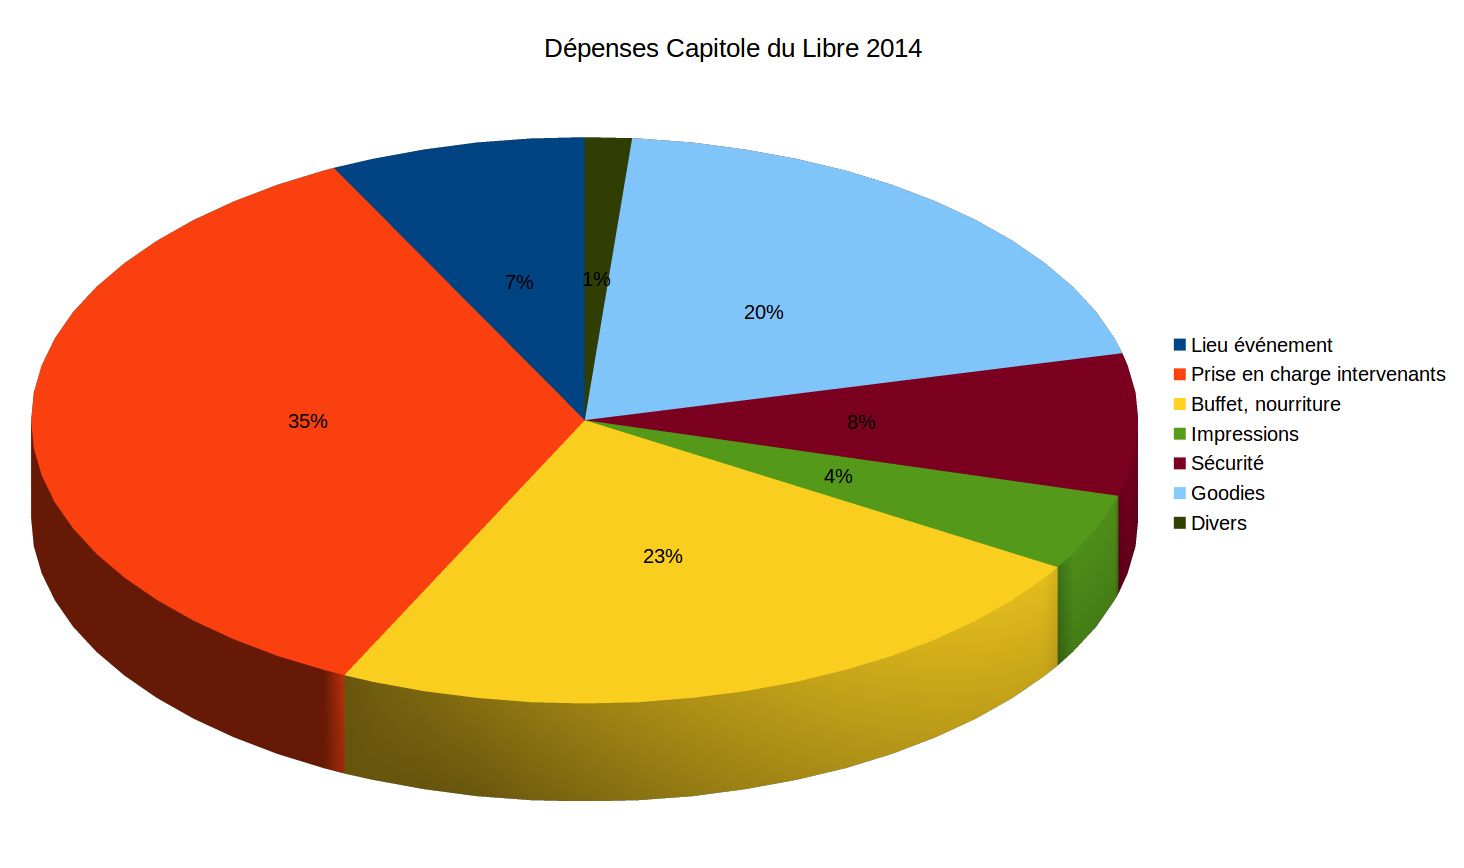
\includegraphics[scale=0.6]{Images/budget_2014.png}\\

Pour l'édition 2015 du Capitole du Libre, nous prévoyons une augmentation de notre budget à \SI{18000}{€} afin principalement :
\begin{itemize}[label=$\bullet$]
\item d'augmenter la superficie de l'événement ;
\item de permettre de faire venir plus d'orateurs afin de continuer à améliorer la qualité et la variété de nos orateurs ;
\item de proposer un buffet dinatoire le samedi soir. Ce buffet ouvert à tous et à participation libre étant un lieu d'échange privilégié lors de ce week-end où se retrouvent orateurs, sponsors et participants.
\end{itemize}

\Separateur

Le détail des dépenses et des recettes du Capitole du Libre 2015 est détaillé dans les deux tableaux respectifs \ref{tab_dépenses} et \ref{tab_recettes} ci-dessous.

\begin{table}[!h]
\begin{center}
	\caption{Dépenses du Capitole du Libre 2015}\label{tab_dépenses}
    \begin{tabular}{|l|c|}
        \hline Dépense & Montant \\
        \hline \textbf{Défraiements intervenants} & \textbf{\SI{5000}{€}} \\
        \hline Déplacements intervenants & \SI{3500}{€} \\
        \hline Hébergement intervenants & \SI{1500}{€} \\
        \hline \textbf{Hébergement manifestation} & \textbf{\SI{3000}{€}}\\
        \hline Chauffage & \SI{1500}{€} \\
        \hline Sécurité & \SI{1500}{€} \\
        \hline \textbf{Apéritif \& Repas} & \textbf{\SI{6000}{€}}\\
        \hline Participation repas intervenants et bénévoles & \SI{1500}{€} \\
        \hline Buffet samedi soir & \SI{4500}{€} \\
        \hline \textbf{Buvette} & \textbf{\SI{600}{€}}\\
        \hline Viénoiseries bénévoles & \SI{150}{€} \\
        \hline Approvisionnement buvette & \SI{400}{€} \\
        \hline Location machines à café & \SI{50}{€} \\
        \hline \textbf{Goodies} & \textbf{\SI{2800}{€} }\\
        \hline T-Shirt Capitole du Libre 2015 & \SI{1400}{€} \\
        \hline Goodies autres & \SI{1400}{€} \\
        \hline \textbf{Communication} & \textbf{\SI{800}{€}} \\
        \hline Impression Flyers & \SI{100}{€} \\
        \hline Impression Affiches & \SI{100}{€} \\
        \hline Impression Programmes & \SI{500}{€} \\
        \hline Fléchage / Indications & \SI{100}{€} \\
        \hline
        \hline \textbf{TOTAL} & \textbf{\SI{18200.00}{€}} \\
        \hline
    \end{tabular}
\end{center}
\end{table}

\begin{table}[!h]
\begin{center}
    \caption{Recettes du Capitole du Libre 2015}\label{tab_recettes}
    \begin{tabular}{|c|r|}
        \hline Dépense & Montant \\
        \hline Sponsors & \SI{15900.00}{€} \\
        \hline Dons & \SI{300.00}{€} \\
        \hline Ventes buvette & \SI{600.00}{€} \\
        \hline Recette boutique & \SI{1600.00}{€} \\
        \hline \textbf{TOTAL} & \textbf{\SI{18200.00}{€}} \\
        \hline
    \end{tabular}
\end{center}
\end{table}

